\chapter[第一章]{} % (fold)
\label{cha:chapter1}

\section{问题 \\ 舍入误差与有效数字}

设 $S_N = \sum ^N _{j=2} \frac{1}{j^2-1}$,其精确值为 $\frac{1}{2}(\frac{3}{2}-\frac{1}{N}-\frac{1}{N+1})$。

\begin{enumerate}
    \item 编制按从大到小的顺序 $S_N = \frac{1}{2^2-1} + \frac{1}{3^2-1} + ... + \frac{1}{N^2-1}$,计算 $S_N$ 的通用程序;

    \item 编制按从小到大的顺序 $S_N = \frac{1}{N^2-1} + \frac{1}{(N-1)^2-1} + ... + \frac{1}{2^2-1}$,计算 $S_N$ 的通用程序;

    \item 按两种顺序分别计算 $S_{10^2}$、$S_{10^4}$、$S_{10^6}$,并指出其有效位数(编程时用单精度);

    \item 通过本上机题你明白了什么?

\end{enumerate}

\section{分析}

对于 $\frac{1}{N^2-1}$,当 $N$ 很大时,$\frac{1}{N^2-1}$ 接近0,因此如果按从大到小的顺序计算 $S_N = \frac{1}{2^2-1} + \frac{1}{3^2-1} + ... + \frac{1}{N^2-1}$,由于计算机的舍入误差,会出现\textbf{大数吃小数}的情况,从而比真实结果略小;而如果按从小到大的顺序计算 $S_N = \frac{1}{N^2-1} + \frac{1}{(N-1)^2-1} + ... + \frac{1}{2^2-1}$,其结果应该更加接近真实值。

\section{程序}

q1-1.cpp

\begin{lstlisting}[style = cpp]
#include <iostream>
#include <iomanip>
#include <math.h>

float f(int N) {
    float res = 0;
    res = float(1.0)/(pow(float(N), float(2)) - 1);
    return res;
}

float SN_1(int N) {
    float sum = 0;
    for (int i = 2; i <= N; i++)
    {
        sum += f(i);
    }
    return sum;
}

float SN_2(int N) {
    float sum = 0;
    for (int i = N; i >= 2; i--)
    {
        sum += f(i);
    }
    return sum;
}

float SN_Real(int N) {
    float sum = 0;
    sum = 0.5*(1.5 - 1/N - 1/(N+1));
    return sum;
}

int main() {
    float data0 = 0;
    float data1 = 0;
    float data2 = 0;

    int N = 0;

    std::cout<<"请输入N:"<<std::endl;
    std::cin>>N;

    data0 = SN_Real(N);
    data1 = SN_1(N);
    data2 = SN_2(N);

    std::cout<<"N\t精确值\t\t从大到小\t误差1   \t从小到大\t误差2"<<std::endl;
    std::cout<<N<<"\t"<< std::fixed << std::setprecision(8)<<data0<<"\t"<<data1<<"\t"<<abs(data0-data1)<<"\t"<<data2<<"\t"<<abs(data0-data2)<<std::endl;

    return 0;
}
\end{lstlisting}

\section{算例}

\begin{enumerate}
    \item $S_{10^2}$

    \begin{lstlisting}[style = cpp]
请输入 N: 100
准确值:	0.7399495244
正向求和:	0.7400494814, 误差: 0.0000999570
反向求和:	0.7400495410, 误差: 0.0001000166
    \end{lstlisting}

    \item $S_{10^4}$

    \begin{lstlisting}[style = cpp]
请输入 N: 10000
准确值:	0.7498999834
正向求和:	0.7498521209, 误差: 0.0000478625
反向求和:	0.7498999834, 误差: 0.0000000000
    \end{lstlisting}

    \item $S_{10^6}$

    \begin{lstlisting}[style = cpp]
请输入 N: 1000000
准确值:	0.7499989867
正向求和:	0.7498521209, 误差: 0.0001468658
反向求和:	0.7499990463, 误差: 0.0000000596
    \end{lstlisting}

    \item 从 $10^2 \sim N$ 将两种方式计算的误差曲线绘制出来 (为了观察变化趋势,误差没有取绝对值):

    \begin{figure}[ht]
    \centering
        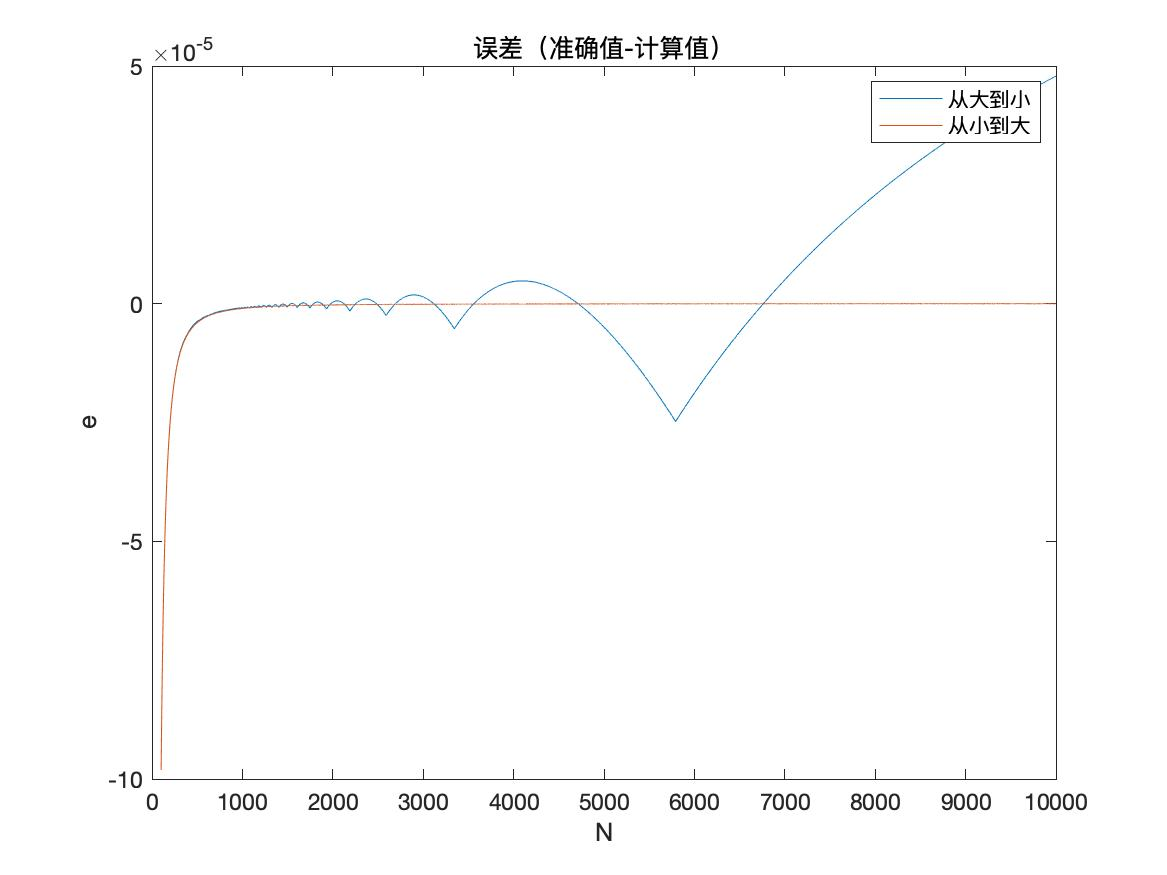
\includegraphics[width=0.8\textwidth]{e10000}
        \caption{两种计算方法的误差对比, N = 10000}
        \label{fig:e10000}
    \end{figure}

\end{enumerate}

\section{结论}

\begin{table}[ht]
  \centering
  \caption{有效位数}
  \label{tab:1}
  \begin{tabular}{*{20}c}
     \hline
    %  \cline{col1-col2}
     N & $10^2$ & $10^4$ & $10^6$ \\
     \hline
     % after \\: \hline or \cline{col1-col2} \cline{col3-col4} ...
     从大到小 & 3  & 4  & 3 \\
     从小到大 & 3  & 7  & 6 \\
     \hline
   \end{tabular}
\end{table}

\begin{enumerate}
    \item 编程证明了之前的分析,及从大到小求和时,会出现大数吃小数的现象,导致误差偏大。从大到小求和时,由于舍入误差的影响,导致结果不稳定;而从小到大求和结果则比较稳定,可以看到随着 N 的增大,误差逐渐趋于0;

    \item 再次证明了数学上的等价并不意味着数值上的等价,在实际的运算中,舍入误差的影响不可低估,在计算中选择一种好的算法可以使结果更加精确。
\end{enumerate}



% chapter chapter1 (end)